\documentclass[10pt,oneside,onecolumn,letterpaper]{article}
\usepackage{graphicx}
\usepackage{xcolor}
\usepackage[hidelinks]{hyperref}
\usepackage{booktabs}
\usepackage{adjustbox}

\usepackage[top=.5in, bottom=1in, left=.5in, right=.7in]{geometry}

\usepackage{fontspec}
\setmainfont{Arial}

\begin{document}

%%
% THIS IS THE HEADER
%%
\noindent\colorbox{black}{
\begin{minipage}[c]{.99\linewidth}
  \vspace{.4cm}
  \Large{\color{white}{\textbf{\hspace{.3cm}University of Massachusetts Boston}}}
  \begin{flushright}
    \vspace{-1.2cm}
    
\includegraphics[width=3cm]{gfx/cs460.png}
  \end{flushright}
\end{minipage}
}

%%
% CONTENT STARTS HERE
%%

\vspace{.5cm} % add some space

\noindent\textbf{CS460 Fall 2019} \\
\textbf{Name:} Jared Barresi \\
\textbf{Student ID:} 00974358 \\
\textbf{Due Date:} 11/11/2019

\section*{Assignment 7: Skinned and Animated Robots!}

\textbf{We will add a mesh to our robot bones and then create an animated crowd.}

\vspace{.5cm} % add some space

\begin{center}
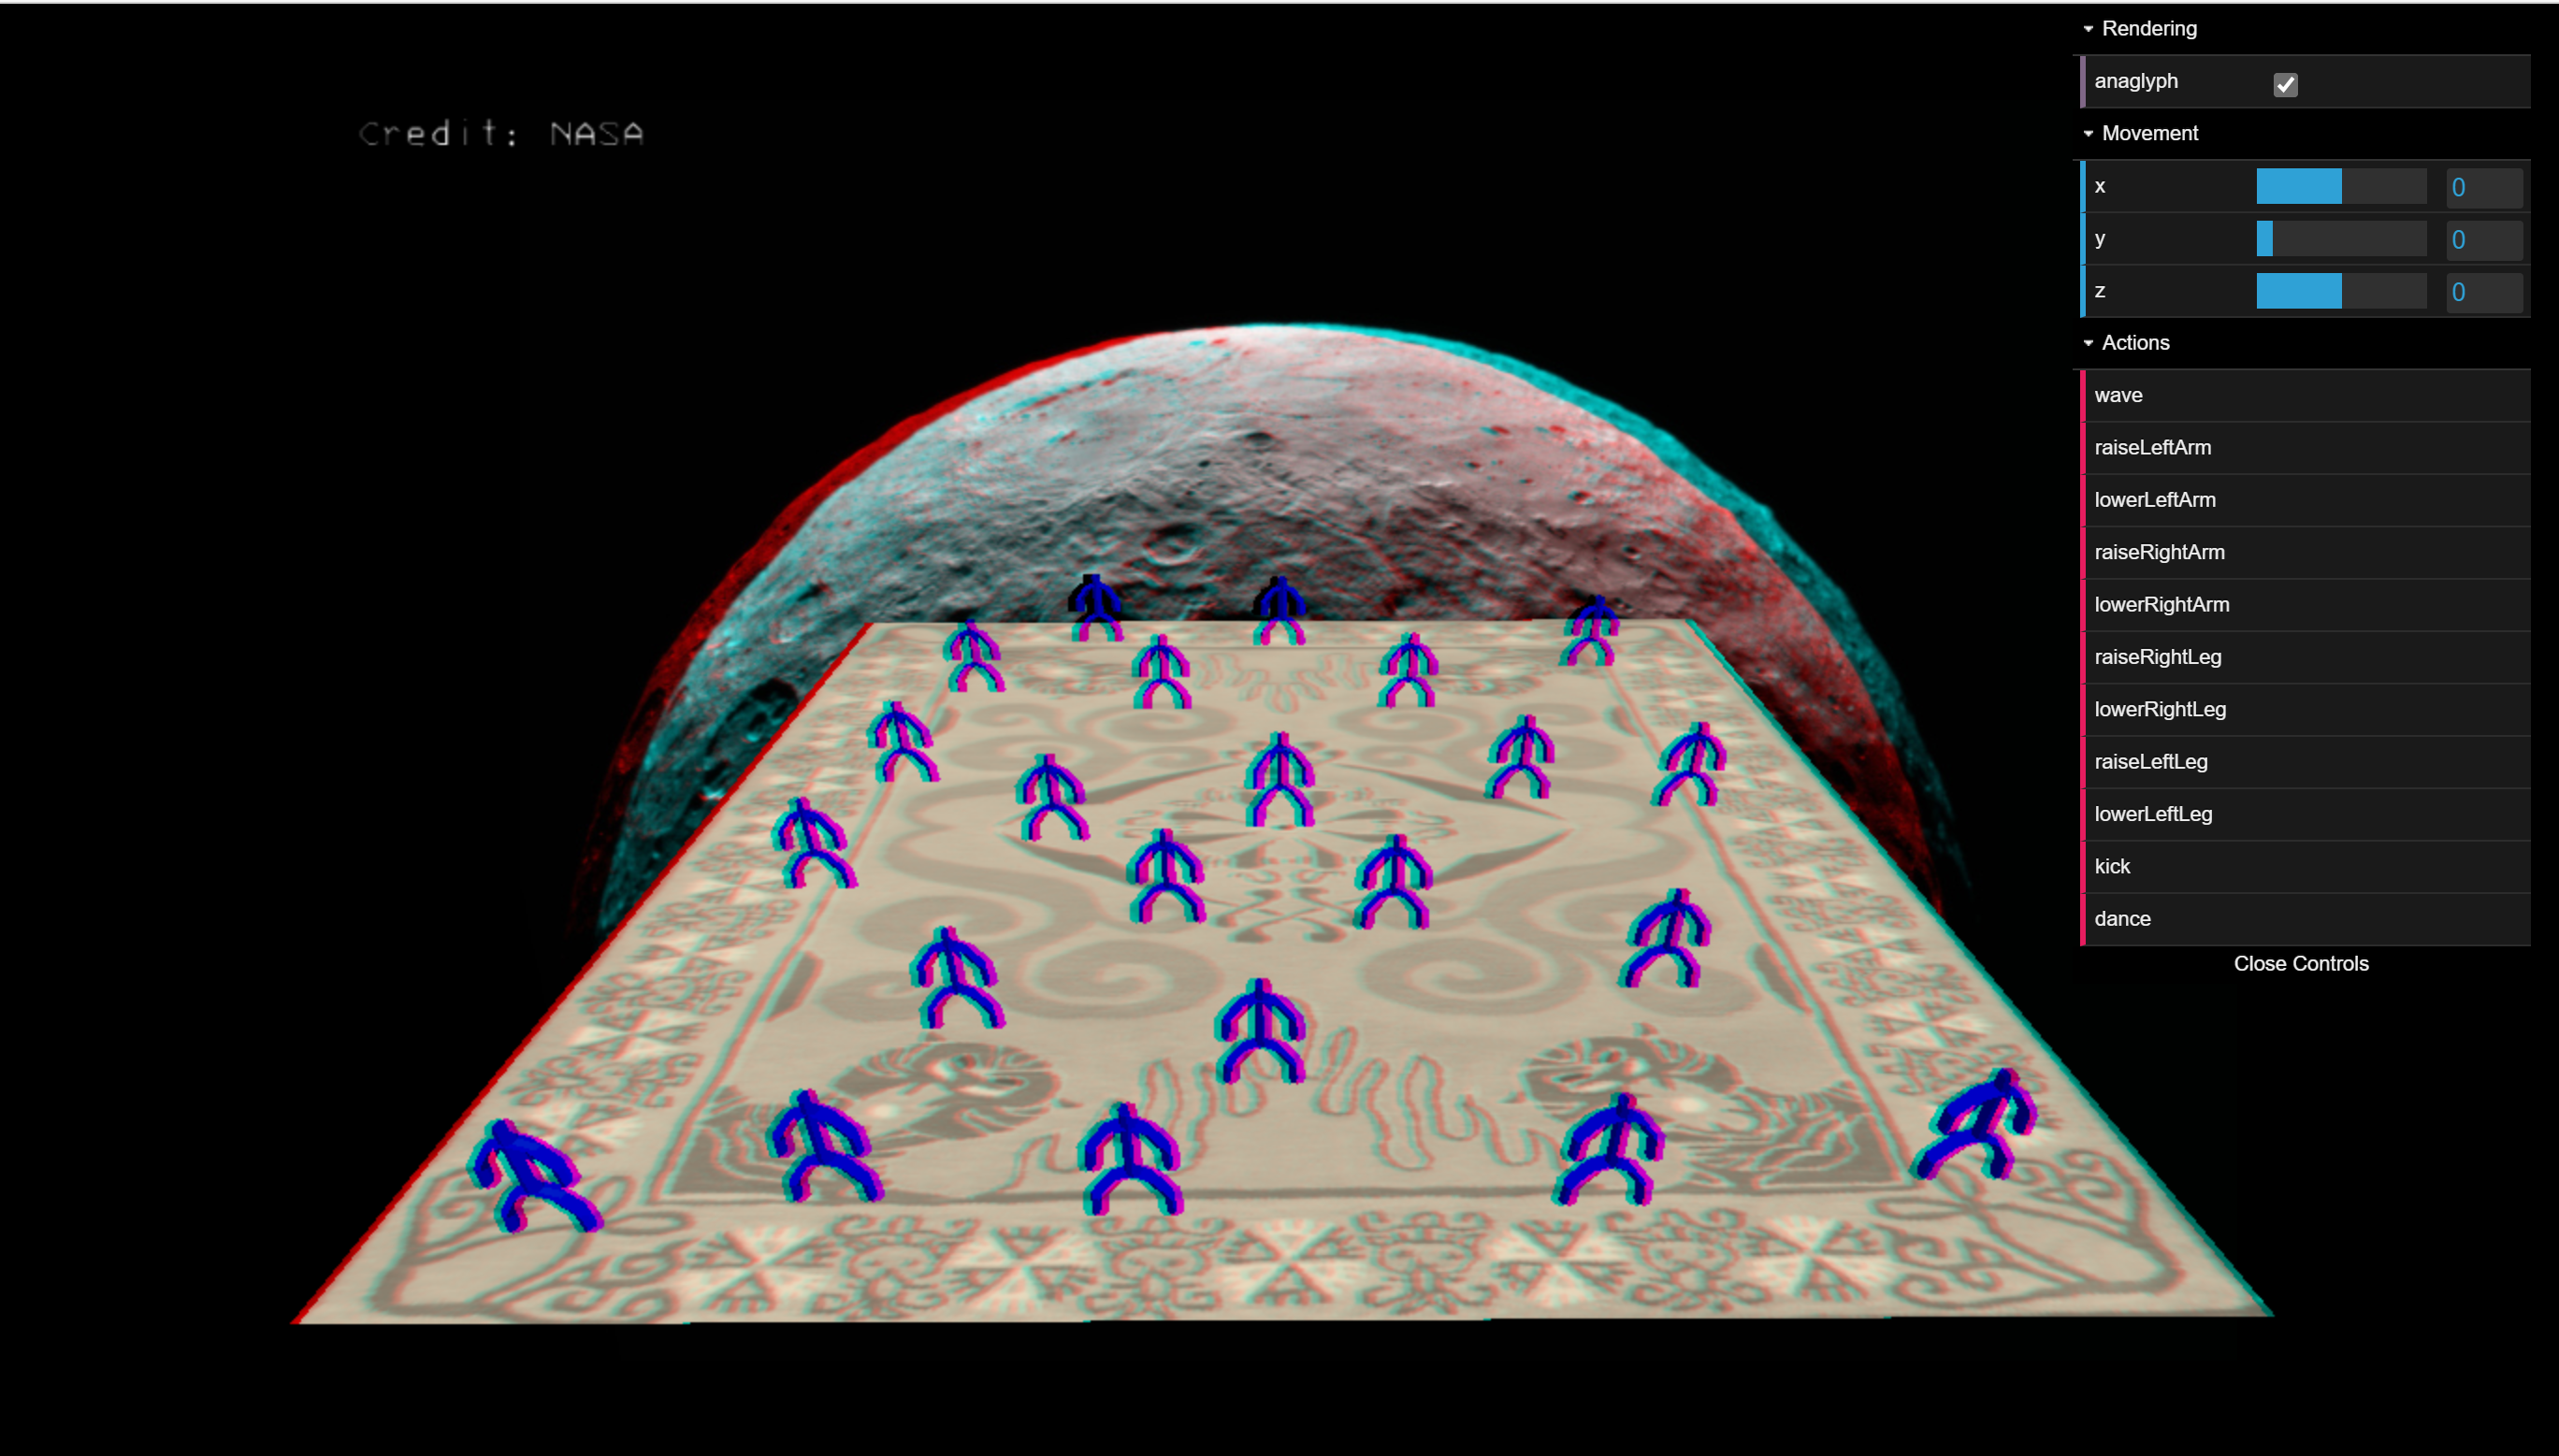
\includegraphics[width=.72\textwidth]{gfx/screenshot-1.png}
\end{center}

\vspace{.5cm}

\noindent\textbf{Starter code for assignment 7.} After pulling from upstream, there is the folder \url{07} in your fork. Please copy \url{index.html} and \url{robot.js} from assignment 6 over or use Daniel's solution from \url{https://cs460.org/shortcuts/28}.  However, we already worked on it during class so your local version might include some of this assignment.

\vspace{.5cm}

\noindent\textbf{Part 1 (50 points):} Please skin the robot using the
\url{HELPER.cylinderSkeletonMesh} function. You will need to call that function 5 times. Note: We started this process in class and there is a work-in-progress \url{robot.js} that can be helpful at \url{https://cs460.org/shortcuts/29/}. Also, the slides around \url{http://slides.com/haehn/cs460_lecture26#/26} explain the HELPER function.

\vspace{.5cm}

\noindent\textbf{Part 2 (30 points):} Allow the placement of multiple robots. Daniel's code includes the \url{THREE.Raycaster} to change the position of a robot when shift+clicked on the floor (see \url{https://cs460.org/shortcuts/28}). Now, rather than changing the position of the robot, we want to create a new one. Please change the code in \url{index.html} to work with \url{robot.js} from part 1.

\vspace{.5cm}

\noindent\textbf{Part 3 (19 points):} Add functionality that allows to animate all placed robots. \textbf{For example, if the user clicks dance, all robots on the floor start dancing.} This can be done using an array as shown in the \url{https://cs460.org/showcase/06} demo from class.

\vspace{.25cm}

\noindent\textbf{Part 4 (1 points):} Please update the screenshot above with your own and then post the github pages url here:

\vspace{.5cm}

\url{https://hltdev8642.github.io/cs460student/07/index.html}

\vspace{3cm}

\noindent\textbf{Bonus (33 points):}

\vspace{.5cm}

\noindent\textbf{Part 1 (18 points):} Please add a head (box or sphere or whatever) to the robot object and use a texture to skin it.
\newline
\noindent\textcolor{blue}{\textit{Visible on load of page}}


\vspace{.5cm}

\noindent\textbf{Part 2 (15 points):} Please add at least one video texture to the scene. And, of course, add some music for the dancing.

\newline
\noindent\textcolor{blue}{\textit{Enable/disable anaglyph checkbox to activate or deactivate video texture}}

\end{document}
